%%%%%%%%%%%%%%%%%%%%%%%%%%%%%%%%%%%%%%%%%%%%%%%%%%%%%%%%%%%%%%%%%%%%%%%%
%                                                                      %
%     File: FormulaStudent.tex           	                           %
%     Tex Master: Thesis.tex                                           %
%                                                                      %
%     Author: Israel Sother                                            %
%     Last modified: 27 May 2024                                       %
%                                                                      %
%%%%%%%%%%%%%%%%%%%%%%%%%%%%%%%%%%%%%%%%%%%%%%%%%%%%%%%%%%%%%%%%%%%%%%%%

\section{Formula Student}

In a formula student competition, two types of evaluation exist, the first category is comprised of static events where the design, cost, and business model of the prototype are analyzed. In the dynamic category, each prototype is evaluated through 5 different events: Skidpad, Acceleration, AutoX, Endurance, and Efficiency (evaluated in the Endurance track), as shown in figure \Cref{fig:fs_tracks}. To be able to compete in dynamic events each prototype needs to pass a series of safety and rule compliance inspections, a process which starts even before de competition with the documentation analysis and finishes with on-site scrutineering.

The Skidpad event is the least relevant for this study as it is designed to test the cornering ability of the vehicle. It is comprised of two circles of radius 9.125m, where the vehicle performs an adaptation first lap and then the lap time is measured on the second lap, when the car is at steady state cornering. As it is a tight and steady course, the power consumption is low not reaching the regulations limit of 80kW, thus the dynamic response and efficiency of the motors have almost no relevance to the performance. 

The acceleration event consists of a standing start 75m straight acceleration, with the maximum battery power limited to 80kw, as it is for all Formula Student events. For this event, the key factors from a powertrain point of view are the torque dynamic response, and how efficiently the powertrain system can deliver power to the ground. 
\begin{figure}[!htb]
	\centering
	% \fbox{
	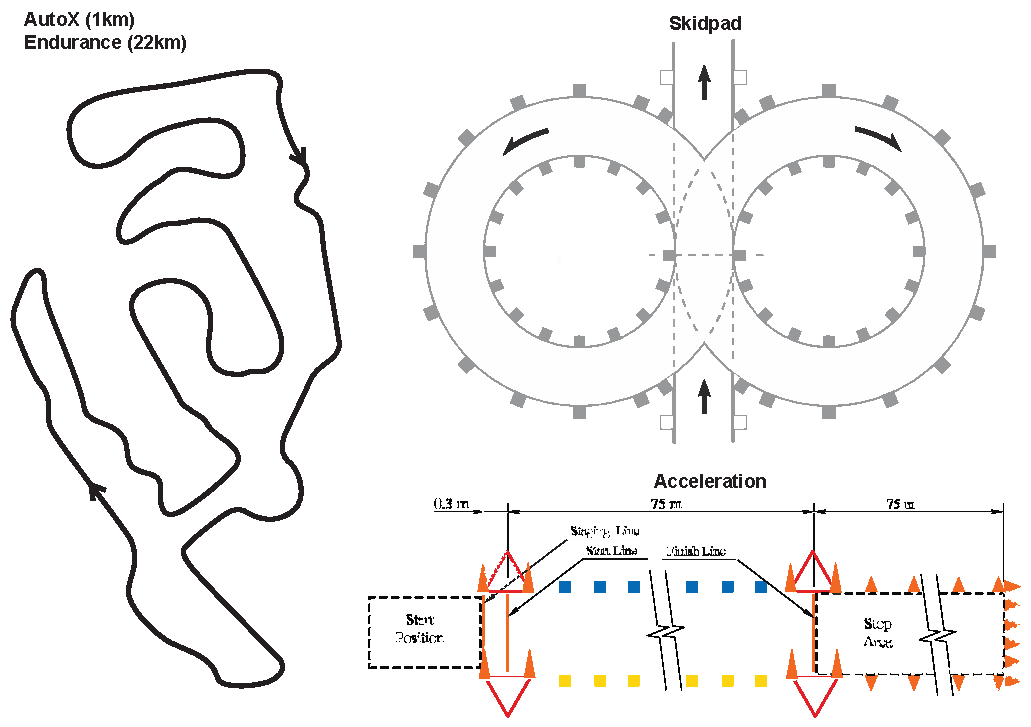
\includegraphics[width=0.8\textwidth]{Figures/Tracks.pdf}
	% }
	\caption[Formula Student Germany Tracks.]{Formula Student Germany Tracks, adapted from~\cite{FSG:rules:2023}.}
	\label{fig:fs_tracks} %chktex 24
\end{figure}
The AutoX is a 1km track with several corners and straights mixed. In this test, an increased dynamic response can delay the braking zone, and the efficiency allows it to reach higher velocities using the same amount of power. Lastly, the endurance event is similar to the AutoX, with enough laps to complete 22km. In this event, although improved dynamics can be beneficial, efficiency is the key factor as it results in more available energy to complete the 22km track while also scoring points in the Efficiency category. 

For the autonomous part of the competition, there are very similar events, with the Skidpad and Acceleration being the same as in the manual mode. The driverless AutoX needs to be a little different, with a smaller distance for the \gls{asr} to be able to see the car throughout the entire track and press the emergency button if necessary. The Endurance event driverless analogous is the TrackDrive event, usually being on the same track as the AutoX, but with fixed 10 laps. Currently, the points performance in the driverless events is mostly dictated by how good the autonomous software is, but as the teams evolve, the cars will play a major role in the results, the same way as it is in the manual category.


Since the FST07, \gls{fst} has used AMK motors and inverters~\cite{amk:DD5-14-10-POW,amk:KW26-S5-FSE-4Q} (datasheets shown in \Cref{chapter:appendixDatasheets}), this set is a good solution for teams switching to a four-motor setup as it is already paired and has good documentation. However, as the team evolves, it is natural to look for improvements, and the AMK inverters were deemed one of the prototypes' current bottlenecks. The use of \gls{igbt} as the switching component, means that this inverter is capped in its switching frequency, using only 8kHz. This low switching frequency reduces powertrain efficiency and increases the set's weight. Another drawback of this solution is the control method as it uses a simple \gls{foc}, thus having a low dynamic response and further reducing efficiency by not using \gls{mtpa} strategies.
A brief outline of the current specification of \gls{fst}'s prototype is shown in \Cref{table:fst13_specs}.

\begin{table}[h]
	\centering
	\caption{FST13 Powertrain Specifications}
	\label{table:fst13_specs}%chktex 24
	\renewcommand{\arraystretch}{1.2} % more space between rows
	% \resizebox{0.85\textwidth}{!}{%
		\begin{tabular}{l l}
			\toprule
			% \rowcolor[HTML]{C0C0C0}
			\textbf{Parameter}                 & \textbf{Value} \\ \toprule
			Battery Voltage Min                & 420 V          \\ \hline
			Battery Voltage Maximum            & 609 V (limited at 600 V by regulations)          \\ \hline
			Battery Voltage Nominal            & 532 V          \\ \hline
			Maximum Power                      & 147 kW (limited at 80 kW by regulations)          \\ \hline
			Number of Motors                   & 4              \\ \hline
			% Motor types		                   & \gls{pmsm}\\ \hline
			% Motor Winding                      & Delta          \\ \hline
			% Motor magnet arrangement           & Spoke          \\ \hline
			Maximum Power per Motor            & 36.75 kW       \\ \hline
			Typical Average Power              & 30 kW          \\ \hline
			Maximum Average Power (1 min)      & 60 kW          \\ \hline
			Maximum Current DC                 & 160 A          \\ \hline
			Maximum motor current RMS (1,24s)  & 105 A          \\ \hline
			AMK Inverter Switching Frequency   & 8 kHz          \\ \hline
			Rotating magnetic field at Maximum Speed   & 1.6 kHz        \\ \hline
			Rated Motor Current                & 41 Arms        \\ \hline
			Rated Motor Voltage                & 350 V          \\ \hline
			% Average Current per phase          & 41             \\ \hline
			% RMS Current per phase              & 2              \\ \hline
			Maximum Speed                      & 20000 RPM      \\ \hline
			Motor Number of Poles              & 10             \\ \hline
			Quadrature Axis Inductance,        & 0.12 mH        \\ \hline
			Direct Axis Inductance             & 0.24 mH        \\ \hline
			Rotor time constant                & 0.01 s         \\ \hline
			Maximum Torque                     & 21 Nm          \\ \hline
			Torque constant                    & 0.26 Nm/Arms   \\ \hline
			Voltage constant                   & 18.8 V/kRPM    \\ \bottomrule
		\end{tabular}
	% }
\end{table}

